\documentclass{standalone}
\usepackage{tikz}
\usepackage{ctex,siunitx}
\usepackage{tkz-euclide}
\usepackage{amsmath}
\usetikzlibrary{patterns, calc}
\usetikzlibrary {decorations.pathmorphing, decorations.pathreplacing, decorations.shapes,}
\begin{document}
\small
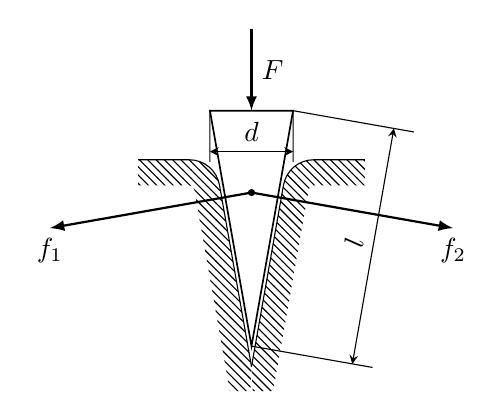
\begin{tikzpicture}[>=stealth,scale=1.3]
  % \useasboundingbox (-0.1,0.1) rectangle(6,-3);
  \fill(0,0)circle(1pt);
  \draw[-latex,thick](0,0)--(190:2)node[below]{$f_1$};
  \draw[-latex,thick](0,0)--(-10:2)node[below]{$f_2$};
  \draw[-latex,thick](0,1.6)--(0,0.8)node[midway,right]{$F$};
  \draw[semithick](-0.406,0.8)--(0,-1.5)--(0.406,0.8)--cycle;
  \draw[thin,<->](-0.406,0.4)--(0.406,0.4)node[midway,above]{$d$};
  \draw[thin](0.406,0.3)--(0.406,0.8)(-0.406,0.3)--(-0.406,0.8)(0,-1.5)--++(-10:1.2)(0.406,0.8)--++(-10:1.2);
  \draw[thin,<->]([shift=(-10:1.0)]0,-1.5)--([shift=(-10:1.0)]0.406,0.8)node[midway,sloped,above]{$l$};
  \fill[pattern =north west lines](0,-1.7)--++(80:1.8)arc(170:90:0.3)--++(0.5,0)--++(0,-0.25)-++(-0.5,0)arc(90:170:0.05)--++(260:2.0)--++(-0.2,0)--cycle;
  \draw(0,-1.7)--++(80:1.8)arc(170:90:0.3)--++(0.5,0);
  \fill[pattern =north west lines](0,-1.7)--++(100:1.8)arc(10:90:0.3)--++(-0.5,0)--++(0,-0.25)-++(0.5,0)arc(90:10:0.05)--++(-80:2.0)--++(0.2,0)--cycle;
  \draw(0,-1.7)--++(100:1.8)arc(10:90:0.3)--++(-0.5,0);
\end{tikzpicture}
\end{document}